\begin{framed}

Objetivos:
\begin{itemize}
    \item Encontrar expresiones para la velocidad, espesor de capa límite y coeficiente de fricción cuando el flujo en la capa límite es turbulento. 
    \item Predecir la separación de la capa límite
\end{itemize}

Contenidos:
\begin{itemize}
    \item Expresiones de capa límite turbulenta para perfil supuesto.
    \item La ley de pared. 
    \item Separación de capa límite.
\end{itemize}

Bibliografía:
\begin{itemize}
    \item Fox, R. W., Pritchard, P. J. y McDonald, A. T. (2009) Introduction to Fluid Mechanics. John Wiley \& Sons. Sección 9.5.
    \item White, F. M. (2006) Viscous Fluid Flow. McGraw-Hill. Tercera edición. Sección 6.4.
\end{itemize}
\end{framed}

\section*{Capa límite turbulenta}

En clases anteriores hemos estado analizando la capa límite de diferentes maneras usando von Kármán, Blasius, Flakner-Skan, y considerando succión y soplido.
Todos estos análisis tienen una cosa en común: la capa límite es considerada laminar.
Ya vimos también que el número de Reynolds en el caso de placa plana es variable en el espacio, y va subiendo a medida que nos movemos por la placa ($Re_x=U_\infty x/\nu$).
Ya sabemos que a medida que crece el número de Reynolds, el flujo se torna inestable, y ante cualquier perturbación se desencadena la transición a turbulencia.
Debido a esto, en la capa límite sobre una placa plana tendremos coexistirá flujo laminar (al incio de la placa) y flujo turbulento (aguas abajo), y en general se considera el Reynolds crítico como $Re_{cr} = 5\cdot10^{5}$.
Un ejemplo de esto se ve en la Figura \ref{fig:capa_limite_Re}, donde la capa límite se pega un salto cuando pasa de laminar a turbulenta, y en la parte turbulenta aparece una región denominada subcapa viscosa o laminar.
%
\begin{figure}
\centering
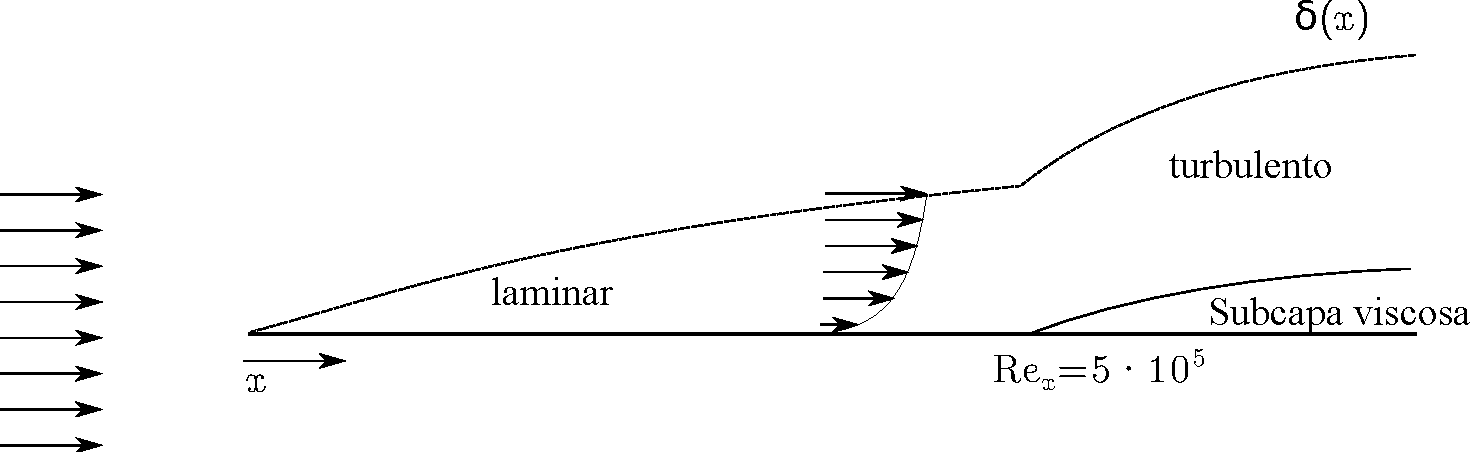
\includegraphics[width=0.9\textwidth]{clase09/capa_limite_Re.pdf}
\caption{Representación gráfica de la capa límite y su transición a turbulencia.}
\label{fig:capa_limite_Re}
\end{figure}

En esta clase vamos a analizar la capa límite turbulenta más en detalle.

\subsection*{Perfil de velocidad dado}

Así como vimos hace algunas clases cuando estudiamos turbulencia, sabemos que el perfil de velocidades va a ser bastante más desordenado en el caso laminar.
Es más, la velocidad va a ir variando con respecto a un promedio $\overline{u}$ debido a fluctuaciones turbulentas $u'$\footnote{Vean el siguiente video desde el minuto 18:40: \url{https://www.youtube.com/watch?v=wMxK2GtFFq0}}, lo que hace muy difícil su análisis.

Experimentalmente, se ha visto que la velocidad promedio de la capa límite turbulenta se acerca mucho a un perfil $y^{1/7}$, más específicamente:
%
\begin{equation}\label{eq:perfil_turbulento}
\frac{u}{U_\infty} = \left(\frac{y}{\delta}\right)^{1/7}.
\end{equation}
%
La Figura \ref{fig:capa_limite_turbulenta} compara la capa límite de Blasius, von Kármán ($\sim y^2$) y turbulenta ($\sim y^{1/7}$), donde el punto negro denota donde está el fin de la capa límite. Como pueden ver, el perfil turbulento tiene una gradiente mucho mayor al perfil laminar cerca de la pared, por lo tanto, el esfuerzo de pared ($\tau_w$) será mayor.
Cabe destacar que este no es un gran modelo cerca del fin de la capa límite, donde la gradiente no permite una transición suave al flujo uniforme al infinito.
%
\begin{figure}
\centering
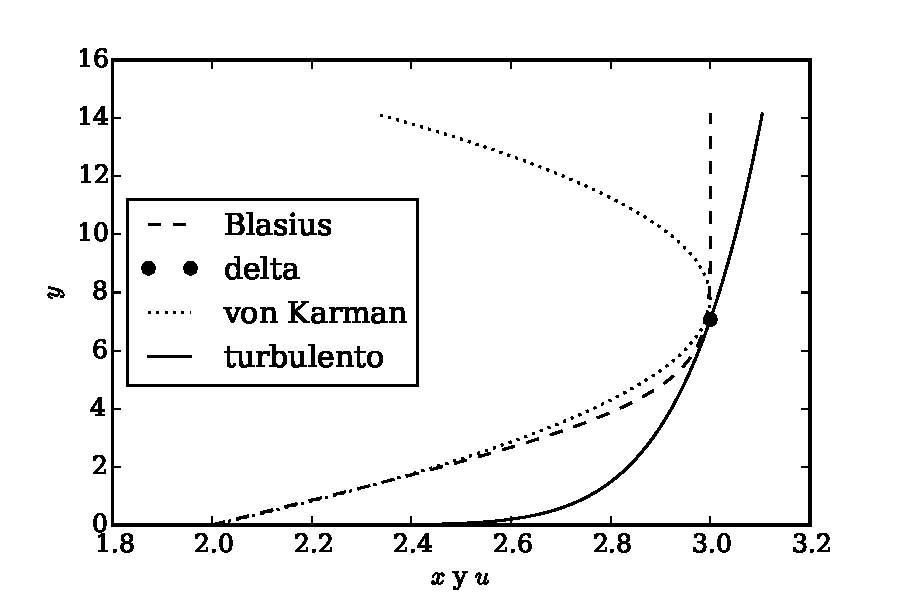
\includegraphics[width=0.6\textwidth]{clase11/capa_limite_turbulenta.pdf}
\caption{Perfil de capa límite laminar (Blasius y von Kármán) y turbulenta.}
\label{fig:capa_limite_turbulenta}
\end{figure}

Durante las últimas clases, hemos estado buscando expresiones para $\delta$, $\delta^*$, $\theta$ y $C_f$ para cada forma de modelar la capa límite. 
Esta no es la excepción, e intentaremos encontrar estas expresiones para el caso turbulento.
Debido a que estamos asumiendo un perfil de velocidades, este análisis debiese ser equivalente al de von Kármán cuando asumimos el perfil parabólico.
En ese caso, igualamos los esfuerzos de pared calculados con la relación integral de von Kármán:
%
\begin{equation}
\tau_w = \rho U_\infty^2 \frac{d\theta}{dx}
\end{equation}
%
donde $\theta$ es el espesor de momentum, a la ecuación de Newton $\tau_w = \left.\mu\frac{du}{dy}\right|_0$, sin embargo, al sacar la derivada de la Ec. \eqref{eq:perfil_turbulento} obtenemos
%
\begin{equation}
\tau_w = \left.\mu \frac{d}{dy}\left(U_\infty\frac{u}{\delta}\right)^{1/7}\right|_0 = \left.\frac{U_\infty\mu}{\delta^{1/7}}y^{-6/7}\right|_0 = \infty.
\end{equation}
%
Claramente, tenemos un problema con el perfil escogido, y vamos a tener que sacar $\tau_w$ de otra manera.
La forma más fácil es hacer un símil con flujo en tuberías
